\clearpage
\phantomsection

\setcounter{chapter}{0}
\chapter[MÔ HÌNH KÊNH VÀ CÁC PHƯƠNG PHÁP NHẬN DẠNG HỆ THỐNG TRONG MIMO KÍCH THƯỚC LỚN]{Mô hình kênh và các phương pháp nhận dạng hệ thống trong MIMO kích thước lớn}
\label{sec:back}

\section{Mô hình kênh trong hệ thống MIMO kích thước lớn}
\label{sec:channel_model}

% Mô hình hoá kênh là quá trình mô hình hóa và đặc trưng hóa các kênh truyền thông không dây để hiểu và dự đoán hiệu suất truyền thông của hệ thống. Trong các hệ thống mMIMO, việc mô hình hoá kênh đóng một vai trò quan trọng để đảm bảo hiệu suất và hiệu quả hoạt động của hệ thống. Có thể kể đến một số lợi ích của một hình kênh truyền tốt (giống với việc truyền thông thực) như sau: hiểu và phân tích kênh truyền vô tuyến; thiết kế hệ thống và cấu hình ăng-ten phù hợp; đánh giá hiệu suất truyền thông; hay phát triển và kiểm tra các thuật toán xử lý tín hiệu. Việc xác định đầy đủ các tham số chính của kênh như độ trễ, suy hao, tán xạ, và nhiễu, từ đó tạo ra mô hình số học chính xác phản ánh sự biến đổi không gian và thời gian của kênh truyền luôn là thách thức trong các hệ mMIMO do sự tương tác phức tạp giữa số lượng khổng lồ các phần tử ăng-ten của mảng. 
% \begin{figure}[htb]
%     \centering
%     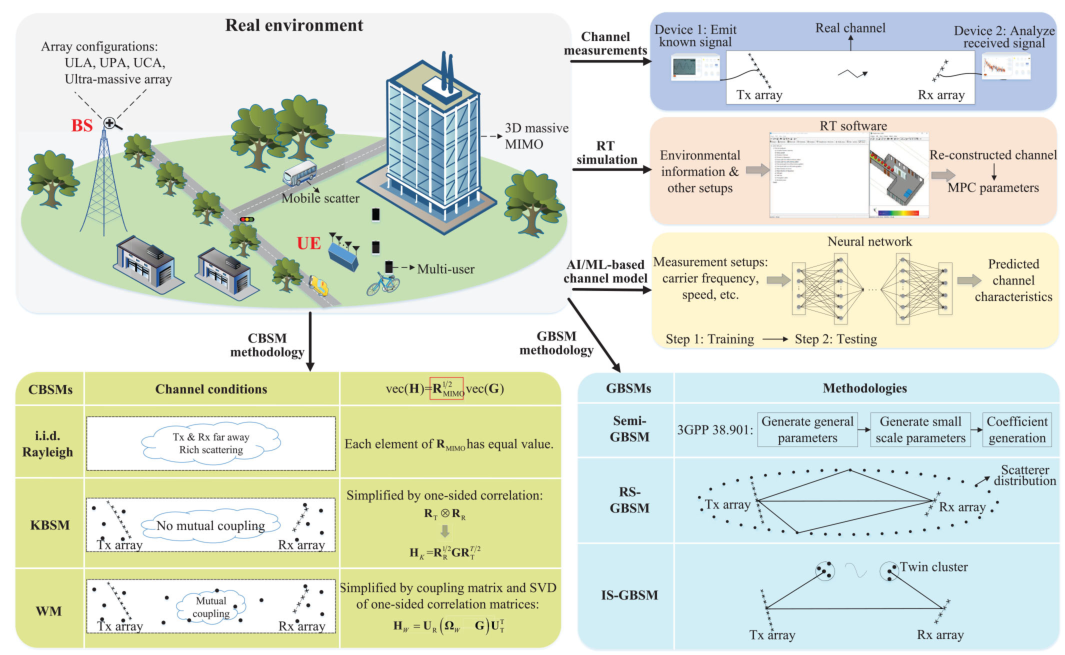
\includegraphics[width=\linewidth]{figures/Fig5.pdf}
%     \caption{Môi trường truyền thông MIMO kích thước lớn và một số mô hình kênh truyền tiêu biểu~\cite{Feng2022}.}
%     \label{fig:channel_model}
% \end{figure}

% Các mô hình kênh truyền MIMO kích thước lớn cũng đã được nhiều tác giả quan tâm nghiên cứu, tổng hợp và phân loại theo những hướng tiếp cận khác nhau như phân loại kênh truyền vật lý/toán học trong~\cite{Almers2007}, kênh xác định/ngẫu nhiên trong~\cite{Wang2018}, hay kênh tiên đoán/không tiên đoán trong~\cite{Feng2022}. Mô hình kênh vật lý biểu diễn kênh dưới dạng các thành phần đa đường trong đó mỗi thành phần được đặc trưng bởi các tham số như biên độ phức, độ trễ, góc đi, góc đến,~\ldots Trong khi đó, mô hình kênh toán học được thiết lập dưới dạng toán học có ma trận kênh với các phần tử là các biến ngẫu nhiên, phụ thuộc nhiều vào kênh và việc sắp đặt hệ thống như băng thông và cấu hình mảng ăng-ten. Mô hình kênh xác định/ngẫu nhiên phụ thuộc vào các tham số trong mô hình là các giá trị cố định hay các biến ngẫu nhiên. Mô hình kênh xác định thường đạt được từ việc giải phương trình Maxwell hay xấp xỉ phương trình truyền sóng trong khi mô hình kênh ngẫu nhiên mô tả các tham số kênh bằng phân bố xác suất. Phương pháp mô hình kênh xác định cho độ chính xác cao hơn nhưng cũng phải trả giá bằng độ phức tạp tính toán. Mô hình kênh tiên đoán dựa trên các thuật toán học máy với khả năng xử lý dữ liệu phi tuyến và tiên đoán để xác định các đặc trưng của kênh truyền. Hình~\ref{fig:channel_model} biểu diễn môi trường truyền thông của mMIMO và một số mô hình kênh truyền tiêu biểu. Nghiên cứu trong~\cite{Wang2018} chỉ ra rằng, vẫn còn sự chồng lấn, hạn chế trong các cách phân loại mô hình kênh truyền hiện nay. Trong luận văn, tác giả quan tâm đến một số mô hình kênh ngẫu nhiên cả vật lý và toán học, cụ thể là mô hình kênh ngẫu nhiên dựa trên tương quan (CBSM - Correlation-based Stochastic Model), mô hình kênh ngẫu nhiên dựa trên hình học (GBSM - Geometry-based Stochastic Model), và mô hình kênh ngẫu nhiên không dựa trên hình học (NGSM - Non Geometry-based Stochastic Model). Các mô hình này sẽ được tìm hiểu kỹ hơn ở những phần tiếp theo của luận văn. 

\subsection{Hệ thống truyền thông mMIMO}
\label{sec:mMIMO}

% \begin{figure}[htb]
%     \centering
%     \begin{tikzpicture}
%         \node[antenna, thick, scale=0.6] at (0, 0) (Tx0) {};
%         \node at (0, 17mm) (text_Tx0) {Tx $0$};
%         \draw[line] (-10mm, 0) -- (Tx0) node [pos=0, left] {$\mathbf{s}_0$};

%         \node[antenna, thick, scale=0.6] at (0, -25mm) (Tx1) {};
%         \node at (0, -8mm) (text_Tx1) {Tx $1$};
%         \draw[line] (-10mm, -25mm) -- (Tx1) node [pos=0, left] {$\mathbf{s}_1$};

%         \node[scale=1.5] at (0, -30mm) (dotss) {$\mathbf{\vdots}$};

%         \node[antenna, thick, scale=0.6] at (0, -55mm) (TxT) {};
%         \node at (0, -38mm) (text_TxT) {Tx $T-1$};
%         \draw[line] (-10mm, -55mm) -- (TxT) node [pos=0, left] {$\mathbf{s}_{T-1}$};

%         \node[antenna, thick, scale=0.6] at (70mm, 0) (Rx0) {};
%         \node at (70mm, 17mm) (text_Rx0) {Rx $0$};
%         \draw[line] (80mm, 0) -- (Rx0) node [pos=0, right] {$\mathbf{x}_{0}$};

%         \node[antenna, thick, scale=0.6] at (70mm, -25mm) (Rx1) {};
%         \node at (70mm, -8mm) (text_Rx1) {Rx $1$};
%         \draw[line] (80mm, -25mm) -- (Rx1) node [pos=0, right] {$\mathbf{x}_{1}$};

%         \node[scale=1.5] at (70mm, -30mm) (dotss) {$\mathbf{\vdots}$};

%         \node[antenna, thick, scale=0.6] at (70mm, -55mm) (RxL) {};
%         \node at (70mm, -38mm) (text_RxL) {Rx $L - 1$};
%         \draw[line] (80mm, -55mm) -- (RxL) node [pos=0, right] {$\mathbf{x}_{L-1}$};

%         \draw[arrow] (3mm, 6mm) -- (67mm, 6mm);
%         \draw[arrow] (3mm, 5mm) -- (67mm, -20mm);
%         \draw[arrow] (3mm, 4mm) -- (67mm, -49mm);

%         \draw[arrow] (3mm, -19mm) -- (67mm, 5mm);
%         \draw[arrow] (3mm, -20mm) -- (67mm, -21mm);
%         \draw[arrow] (3mm, -21mm) -- (67mm, -50mm);

%         \draw[arrow] (3mm, -49mm) -- (67mm, 4mm);
%         \draw[arrow] (3mm, -50mm) -- (67mm, -22mm);
%         \draw[arrow] (3mm, -51mm) -- (67mm, -51mm);

%         \node at (35mm, -60mm) (H) {$\mathbf{H} \in \mathbb{C}^{L \times T}$};
%     \end{tikzpicture}
%     \caption{Hệ thống truyền thông mMIMO.}
%     \label{fig:sys_model}
% \end{figure}

Xem xét một mô hình hệ thống thu phát mMIMO đơn giản với $T$ ăng-ten phát và $L$ ăng-ten thu. Hệ thống được biểu diễn dưới dạng toán học tại thời điểm $n$ như sau: 
\begin{equation}
\label{eq:timedomain}
    \mathbf{x}(n) = \mathbf{H}(n)*\mathbf{s}(n) + \mathbf{w}(n)
\end{equation}
trong đó $\mathbf{s}(n) \in \mathbb{C}^{T \times 1}$ là các ký hiệu được gửi đi từ $T$ bộ phát, ma trận $\mathbf{H} \in \mathbb{C}^{L\times T}$ biểu diễn kênh truyền, $\mathbf{x}(n) \in \mathbb{C}^{L \times 1}$ là véc-tơ biểu diễn tín hiệu thu được từ $L$ ăng-ten, và $\mathbf{w} \in \mathbb{C}^{L \times 1}$ là nhiễu cộng tính (AWGN).
Trong trường hợp kênh là pha-đinh phẳng tần số, còn được gọi là kênh băng hẹp thì phương trình~(\ref{eq:timedomain}) trở thành:  
\begin{equation}
    \mathbf{x}(n) = \mathbf{H}(n)\mathbf{s}(n) + \mathbf{w}(n)
\end{equation}
Các phần tử trong ma trận kênh được biểu diễn bởi các biến ngẫu nhiên phức có pha thường được mô hình bởi phân bố đều và phân bố biên độ tùy thuộc môi trường.


\subsection{Mô hình kênh CBSM}
Mô hình kênh CBSM thuộc loại mô hình kênh toán học, ngẫu nhiên.
Xét hệ mMIMO bất biến với thời gian có mô hình kênh hoàn chỉnh biểu diễn bởi phương trình~(\ref{eq:unstructure}).
\begin{equation}
    \label{eq:unstructure}
    \mathbf{H}_{total} = \beta \mathbf{H} 
\end{equation}
trong đó, $\beta$ đại diện cho ảnh hưởng của pha-đinh kích thước lớn gồm suy hao do khoảng cách truyền, pha-đinh bóng mờ, hiệu ứng chặn, và hấp thụ khí quyển; ma trận $\mathbf{H}$ đại diện cho ảnh hưởng của pha-đinh kích thước nhỏ, không có tia nhìn thẳng (NLOS). Xét ảnh hưởng của pha-đinh kích thước nhỏ, ma trận $\mathbf{H}$ được biểu diễn như sau:
\begin{equation}
    \mathbf{H} = \begin{bmatrix}
    h_{0,0} & \ldots  & h_{0, T-1} \\ 
    \vdots & \ddots & \vdots\\ 
    h_{L-1, 0} & \ldots  & h_{L-1, T-1}
    \end{bmatrix}
\end{equation}
với mỗi phần tử $h_{l,t}$ tương ứng là đáp ứng xung của kênh giữa ăng-ten phát thứ $t$ và ăng-ten nhận thứ $l$ (có thể dùng cho mô hình kênh băng rộng). 
Mô hình kênh được chia thành 2 loại: mô hình không tương quan và mô hình tương quan. Xét ma trận hiệp phương sai của ma trận kênh như sau:
\begin{equation}
    \label{eq:1.6}
    \mathbf{R}_{\mathbf{H}} = \mathbb{E} ({\operatorname{\mathbf{H}} \operatorname{\mathbf{H}}^H})
\end{equation}
với $(.)^H$ là phép biến đổi Hermitian.

Với mô hình kênh không tương quan, các phần tử của ma trận kênh được coi là có phân bố giống nhau và độc lập (i.i.d) hay hàm hiệp phương sai của ma trận kênh là một ma trận đường chéo với các giá trị đường chéo thường bằng 1. Với mô hình ma trận kênh i.i.d Rayleigh sẽ có các phần tử là các biến ngẫu nhiên Gauss phức trung bình bằng 0, phương sai bằng 1.


% \begin{equation}
%     \label{eq:correlation}
%     \operatorname{vec}(\mathbf{H}) = \mathbf{R}^{1/2}_{\mathbf{H}} \operatorname{vec} (\mathbf{G})
% \end{equation}
% trong đó, $\operatorname{vec}$ là phép véc-tơ hoá một ma trận, từ $\mathbf{H}$ kích thước $L\times T$ thành $LT \times 1$. Ký hiệu $\mathbf{G}$ biểu diễn ảnh hưởng của kênh khi không có sự tương quan giữa các phần tử như đã trình bày ở trên, $\operatorname{vec}(\mathbf{G})$ chứa các biến ngẫu nhiên i.i.d Gaussian có kỳ vọng bằng $0$ và phương sai $1$. Ma trận $\mathbf{R}_{\mathbf{H}}$ mô tả cấu trúc không gian của các mảng mMIMO, trong đó xem xét sự tương quan (correlation) lẫn nhau giữa các phần tử trong ma trận kênh truyền. Ma trận này được ước lượng như sau:
% Với mô hình kênh có sự tương quan, ma trận hiệp phương sai kênh~(\ref{eq:1.6}) có độ phức tạp tương ứng với $\mathcal{O}((LT)^2)$, tăng nhanh theo số phần tử ăng-ten trong hệ mMIMO. Phương pháp mô hình ngẫu nhiên Kronecker (KBSM - Kronecker-based Stochastic Model)~\cite{Chuah1998} được đề xuất để giảm thiểu độ phức tạp khi ước lượng $\mathbf{R}_{\mathbf{H}}$. 

% Trong đó, giả sử không có sự tương quan giữa mảng ăng-ten phát và thu, đồng thời không tồn tại các nguồn tán xạ giữa hai mảng ăng-ten này. Ma trận hiệp phương sai $\mathbf{R}_{\mathbf{H}}$ được phân tích thành:
% \begin{equation}
%     \mathbf{R}_{\mathbf{H}} = \mathbf{R}_{\text{tx}} \otimes \mathbf{R}_{\text{rx}}
% \end{equation}
% với $\mathbf{R}_{\text{tx}}$ và $\mathbf{R}_{\text{rx}}$ lần lượt là ma trận tương quan của các phần tử ăng-ten bên phát và thu, $\otimes$ là phép nhân Kronecker. Hai ma trận này lần lượt có dạng $\mathbf{R}_{\text{tx}} = \mathbb{E}(\mathbf{H}^\top \mathbf{H}^*)$ và $\mathbf{R}_{\text{rx}} = \mathbb{E}(\mathbf{H} \mathbf{H}^H)$, với $(.)^\top$ là phép chuyển vị ma trận. Dựa trên cấu trúc hình học của mảng ăng-ten, hai ma trận kể trên được xác định theo~\cite{Kshetrimayum2017}.


% \subsection{Mô hình kênh GBSM}
% \label{sec:GBSM}
% GBSM thuộc loại mô hình kênh vật lý có độ phức tạp cao. Mô hình này xem xét sự lan truyền của sóng vô tuyến trong không gian dưới dạng các cụm (cluster), tia/đường truyền riêng biệt. Việc xây dựng mô hình có thể dựa hoàn toàn trên dạng hình học của các phần tử tán xạ như mô hình RS-GBSM (Regular shaped - GBSM) có các tán xạ nằm trên các hình phổ biến như 1 vòng, 2 vòng, elíp,~\ldots, hay mô hình IS-GBSM (Irregular shaped - GBSM) với các tán xạ nằm trên các đường hình học không phổ biến như mô hình 2 cụm thể hiện đặc tính không dừng trong không gian của kênh mMIMO,~\ldots Ngoài ra, mô hình kênh Semi-GBSM cũng được sử dụng rất nhiều trong các chuẩn truyền thông di động. Ví dụ như: 3GPP phiên bản 16~\cite{r16} cho 5G hay WINNER II~\cite{WINNER}. So với GBSM, Semi-GBSM mặc dù có độ chính xác và khả năng mở rộng tốt hơn nhưng mô hình này lại có độ phức tạp lớn hơn nhiều do mô hình kênh không chỉ được xây dựng từ thông tin hình học của các cluster và phân bố của các tán xạ mà còn dựa trên môi trường được định nghĩa bởi người dùng, layout mạng và và thông số của mảng ăng-ten~\cite{Zhu2022}.
% %\begin{figure}[htb]
% %    \centering
% %    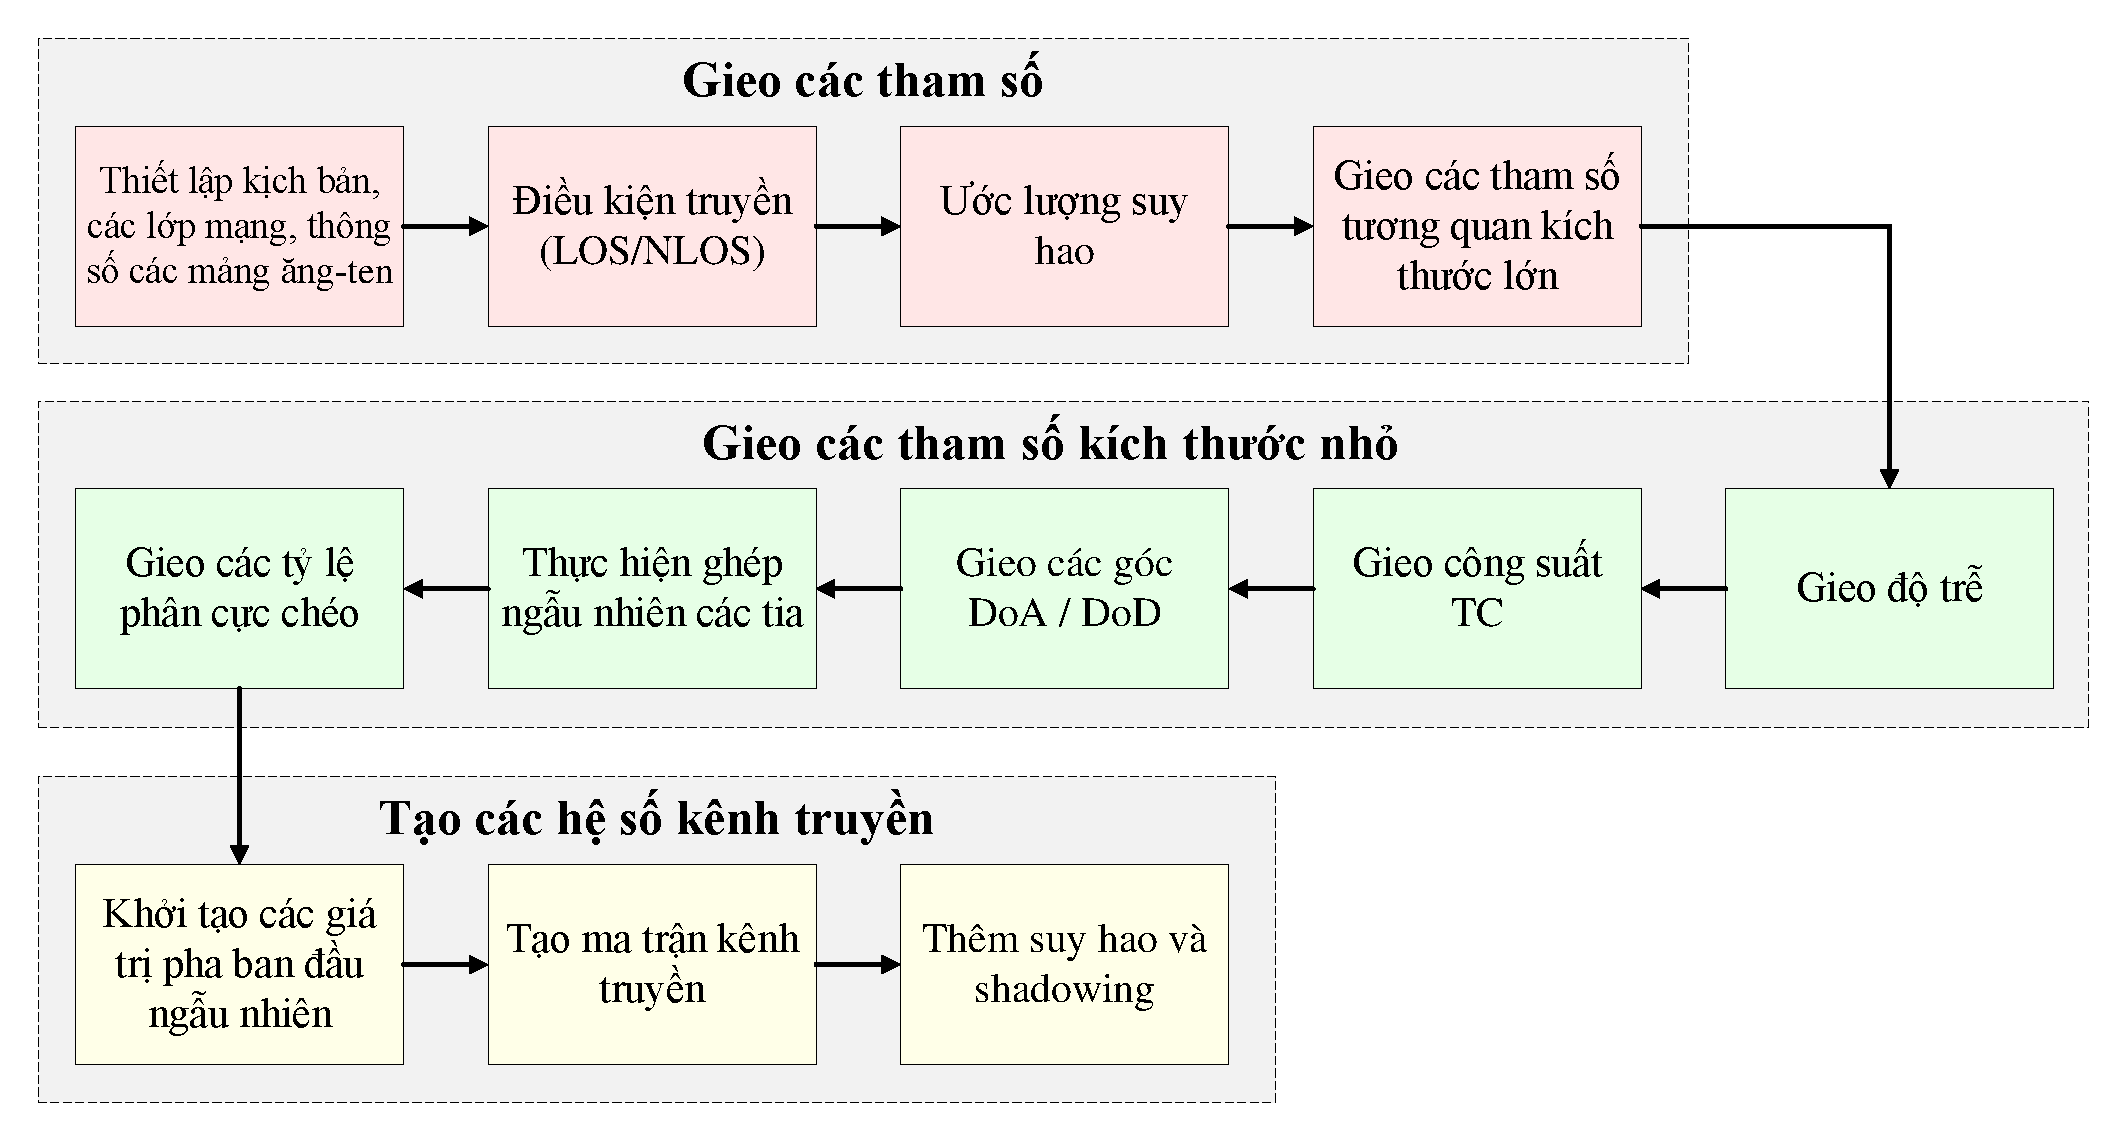
\includegraphics[width=\linewidth]{figures/3GPP_flow.pdf}
% %    \caption{Các bước tạo mô hình kênh truyền trong tiêu chuẩn 3GPP phiên bản 16~\cite{r16}.}
% %    \label{fig:3gpp_flow}
% %\end{figure}

% % Trên hình~\ref{fig:3gpp_flow} là 12 bước trong quá trình mô hình hoá kênh truyền mMIMO được đề ra trong tiêu chuẩn 3GPP phiên bản 16 dành cho các hệ thống 5G. Phần tiếp theo sẽ trình bày sơ lược về các nét chính trong phương pháp mô hình hoá này. 
% Theo mô hình GBSM, phần tử của ma trận kênh được tính bởi~\cite{Ju2021}:
% \begin{equation}
%     \label{eq:3gpp}
%     \begin{aligned}
%         {h}_{l, t}(n) = \sum\limits_{m=0}^{M-1} \sum\limits_{k=0}^{M_n - 1} \beta_{m, k, t} & \cdot e^{i\varphi_{m, k, t}} \cdot \delta\left(n-\tau_{m, k, t}\right) \\
%         &\cdot e^{-i k_s s_t(\theta^d_{m, k, t}, \phi^d_{m, k, t})} \cdot
%         e^{-i k_s s_l(\theta^a_{m, k, t}, \phi^a_{m, k, t})} 
%     \end{aligned}
% \end{equation}
% $M, M_n$ lần lượt là số lượng các cụm và số lượng các tia trong mỗi cụm đến bên thu. Với tia thứ $k$ trong cụm thứ $m$, các ký hiệu $\beta, \varphi, \tau$ đại diện cho biên độ, pha, và thời gian trễ tuyệt đối của mỗi tia. Góc ngẩng (zenith), góc phương vị (azimuth) của hướng sóng đi (DoD - Direction of Departure) và hướng sóng đến (DoA - Direction of Arrival) được ký hiệu lần lượt là $\theta^d, \phi^d, \theta^a$, và $\phi^a$. Ký hiệu $(\cdot)$ tương ứng là phép nhân vô hướng. Các thành phần biên độ $\beta_{m,k,t}$ của $h_{l, t}$ phụ thuộc vào suy hao, như một hàm của tần số sóng mang $f_c$, khoảng cách giữa ăng-ten phát và ăng-ten thu $d$, cho bởi:
% \begin{equation}
%     \label{eq:FSPL}
%     \begin{aligned}
%         \beta_{m, k, t}(f_c, d)[\mathrm{dB}]=& \mathrm{FSPL}\left(f_c, d_{0}\right)+10 \xi \log _{10}\left(\frac{d}{d_{0}}\right)+\chi_{\sigma}, \\
%         & \text { với } d \geq d_{0}, \text { khi } d_{0}=1\mathrm{m}
%     \end{aligned}
% \end{equation}
% trong đó, $\operatorname{FSPL}\left(f_c, d_{0}\right)=20 \log _{10}\left(4 \pi d_{0} c / f_c\right)$, $c$ là vận tốc ánh sáng, $\xi$ đại diện cho hệ số mất mát hàm mũ (PLE - Path Loss Exponent), và $\chi_{\sigma}$ là đại diện cho hiệu ứng pha-đinh bóng mờ và được mô hình hoá dưới dạng một biến ngẫu nhiên lognormal trung bình bằng 0 và độ lệch chuẩn $\sigma$. 
% Các thông số trong các phương trình (\ref{eq:3gpp}) và (\ref{eq:FSPL}) được quy định và đo đạc xác định cho từng môi trường khác nhau. Đặc trưng của kĩ thuật semi-GBSM là ngoài sử dụng các tham số ngẫu nhiên, rất nhiều tham số của kênh truyền đã được đo lường từ trước và cố định với mỗi điều kiện cụ thể.
% Ví dụ, việc xác định số lượng các TC, trên bảng~\ref{tab:num_TC} chỉ ra các thông số được đo đạc này cho bốn loại môi trường cụ thể, bao gồm: UMi - khu dân cư kích cỡ micro, UMa - khu dân cư kích cỡ macro, RMa - khu nông thông kích cỡ macro, và điều kiện văn phòng trong nhà. Mỗi môi trường trên, các kịch bản đo được thiết lập ở 2 hoặc 3 tình huống gồm: tầm nhìn thẳng (LOS - Line of Sight), không tầm nhìn thẳng (NLOS - Non-LOS), và từ bên ngoài vào trong nhà (O2I - Outdoor to Indoor).
% \begin{table}
% \centering
% \caption{Số lượng các TC và sub-path trong mỗi TC theo chuẩn 3GPP phiên bản 16~\cite{r16}.}
% \label{tab:num_TC}
% \begin{tabular}{|l|c|c|c|c|c|c|} 
% \hline
% \multicolumn{1}{|c|}{\multirow{2}{*}{\textbf{Thông số}}} & \multicolumn{3}{c|}{\begin{tabular}[c]{@{}c@{}}\textbf{UMi - Khu dân cư,}\\\textbf{kích cỡ micro}\end{tabular}} & \multicolumn{3}{c|}{\begin{tabular}[c]{@{}c@{}}\textbf{UMa - Khu dân cư,}\\\textbf{~kích cỡ macro~}\end{tabular}} \\ 
% \cline{2-7}
% \multicolumn{1}{|c|}{} & \textbf{LOS} & \textbf{NLOS} & \textbf{O2I} & \textbf{LOS} & \textbf{NLOS} & \textbf{O2I} \\ 
% \hline
% \textbf{Số lượng TC} & 12 & 19 & 12 & 12 & 20 & 12 \\ 
% \hline
% \textbf{Số lượng sub-path mỗi TC} & 20 & 20 & 20 & 20 & 20 & 20 \\ 
% \hline
% \multicolumn{1}{|c|}{\multirow{2}{*}{\textbf{Thông số}}} & \multicolumn{3}{c|}{\begin{tabular}[c]{@{}c@{}}\textbf{\textbf{RMa - Khu nông thôn,}}\\\textbf{\textbf{~kích cỡ macro~}}\end{tabular}} & \multicolumn{3}{c|}{\begin{tabular}[c]{@{}c@{}}\textbf{\textbf{Văn phòng,}}\\\textbf{\textbf{~trong nhà}}\end{tabular}} \\ 
% \cline{2-7}
%  & \textbf{LOS} & \textbf{NLOS} & \textbf{O2I} & \textbf{LOS} & \multicolumn{2}{c|}{\textbf{NLOS}} \\ 
% \hline
% \textbf{Số lượng TC} & 11 & 10 & 10 & 15 & \multicolumn{2}{c|}{19} \\ 
% \hline
% \textbf{Số lượng sub-path mỗi TC} & 20 & 20 & 20 & 20 & \multicolumn{2}{c|}{20} \\
% \hline
% \end{tabular}
% \end{table}

% Tiếp đến, độ dịch pha ban đầu của các sub-path trong mỗi TC cũng được 3GPP đưa ra như trên bảng~7.5-3 tại tài liệu~\cite{r16}.
% \begin{table}
% \centering
% \caption{Độ lệch pha của các sub-path trong một TC.}
% \label{tab:phase}
% \begin{tabular}{|c|c|c|c|} 
% \hline
% \multicolumn{1}{|c|}{\textbf{sub-path \#}} & \multicolumn{1}{c|}{$\varphi_{n,m,t} (^\circ)$} & \textbf{\textbf{sub-path \#}} & $\varphi_{n,m,t} (^\circ)$ \\ 
% \hline
% 1, 2 & $\pm$ 0,0447 & 11, 12 & $\pm$0,6797 \\ 
% \hline
% 3, 4 & $\pm$ 0,1413 & 13, 14 & $\pm$0,8844 \\ 
% \hline
% 5, 6 & $\pm$ 0,2492 & 15, 16 & $\pm$1,1481 \\ 
% \hline
% 7, 8 & $\pm$ 0,3715 & 17, 18 & $\pm$1,5195 \\ 
% \hline
% 9, 10 & $\pm$ 0,5129 & 19, 20 & $\pm$2,1551 \\
% \hline
% \end{tabular}
% \end{table}
% Thông tin về tỷ lệ công suất của các sub-path trong mỗi TC và độ trễ của chúng so với sub-path đến sớm nhất được trình bày trên bảng~7.5-5 tại tài liệu~\cite{r16}. Cụ thể, mỗi TC sẽ được chia nhỏ hơn nữa thành 3 cụm con (SC - Sub-cluster). Các sub-path sẽ được chia vào một trong ba SC trên dựa trên thời gian trễ của chúng so với tia đến sớm nhất. Bốn thông số còn lại bao gồm $\theta$ và $\phi$ của bên thu và phát được biểu diễn dưới dạng các giá trị ngẫu nhiên thuộc các phân bố khác nhau tuỳ thuộc vào điều kiện môi trường truyền thông, chi tiết xem trong các bảng từ 7.5-6 đến 7.5-10 tại~\cite{r16}.
% \begin{table}
% \centering
% \caption{Thông tin về công suất và độ trễ của các sub-path trong mỗi TC.}
% \label{tab:SC}
% \begin{tabular}{|c|c|c|c|} 
% \hline
% \vcell{\textbf{SC \#}} & \vcell{\textbf{sub-path \#}} & \vcell{\begin{tabular}[b]{@{}c@{}}\textbf{Tỷ lệ công suất}\\\textbf{($\beta_{n, m, t} / \sum_{m=1}^{M} \beta_{n, m, t}$)}\end{tabular}} & \vcell{\begin{tabular}[b]{@{}c@{}}\textbf{Trễ tuyệt đối}\\\textbf{($\tau_{n, m, t} - \tau_{n, 1, t}$)}\end{tabular}} \\[-\rowheight]
% \printcelltop & \printcelltop & \printcelltop & \printcelltop \\ 
% \hline
% 1 & 1, 2, 3, 4, 5, 6, 7, 8, 19, 20 & 10/20 & 0 ns \\ 
% \hline
% 2 & 9, 10, 11, 12, 17, 18 & 6/20 & 5 ns \\ 
% \hline
% 3 & 13, 14, 15, 16 & 4/20 & 10 ns \\
% \hline
% \end{tabular}
% \end{table}


\subsection{Mô hình kênh NGSM}
\label{sec:NGSM}
NGSM là mô hình kênh ngẫu nhiên vật lý không dựa trên phân bố hình học của các nguồn tán xạ, điển hình là mô hình kênh SV (Saleh Valenzuela).
Mô hình kênh SV được đề xuất với độ phức tạp nhỏ hơn nhiều so với mô hình GBSM. 
% Do vậy, mô hình kênh NGSM hiện nay được xem xét dưới dạng là các mô hình tham số (parametric)~\cite{Le2018, Swindlehurst2022}. Mô hình này vẫn kế thừa đặc trưng không gian của GBSM khi xem xét việc truyền sóng theo các đường khác nhau trong không gian 3D (DoA, DoD và cấu trúc mảng ăng-ten được gộp trong $\varphi$).
Cụ thể là: thay vì chia thành các cụm, các tia với các góc, độ trễ khác nhau, mô hình SV gộp các cụm thành các đường truyền lớn với điều kiện xem xét đặc trưng là tính thưa trong các hệ truyền thông sử dụng sóng mi-li-mét. Các thành phần suy hao, dịch pha, và độ trễ được gộp chung lại thành một hệ số khuếch đại phức ($\beta$). Khi đó các phần tử của ma trận kênh được biểu diễn dưới dạng:
\begin{equation}
    h_{l, t} = \sum\limits_{m=0}^{M-1} \beta_{m, t} \cdot e^{\varphi_{l, m, t}} 
\end{equation}
với $\beta$ và $\varphi_l(\theta, \phi)$  là các biến ngẫu nhiên.
Trong chương~\ref{sec:CRB} của luận văn, mô hình kênh truyền này được gọi là ``\textbf{có cấu trúc}'' (structured) để phân biệt với không sử dụng cấu trúc trong CBSM.


\subsection{Đánh giá các phương pháp mô hình kênh cho mMIMO}

Theo đánh giá trong các công bố trước đó đã chỉ ra: kênh xác định cho độ chính xác cao nhưng độ phức tạp tính toán cũng cao và tính tổng quát thấp; kênh CBSM cho cả ba thông số đều thấp nhưng lại rất thuận tiện trong phân tích; và cuối cùng là kênh GBSM cho độ chính xác vừa đủ, độ phức tạp trung bình và tính tổng quát cao.
% chính xác thấp cho tốc độ bít lớn nhất tương đương với mô hình kênh truyền xác định qua đo đạc, do đây cũng là hai phương pháp gần nhất với môi trường truyền thông không dây thực tế. Điểm hạn chế của cả hai phương pháp xác định và GBSM nằm ở độ phức tạp trong các bài toán nghiên cứu. Với trường hợp mô hình kênh như của 3GPP đã được trình bày ở trên, phải cần đến 12 bước theo như tài liệu gốc tại~\cite{r16} để mô hình hoá một kênh truyền cho một điều kiện truyền thông cụ thể duy nhất. Do vậy, hai phương pháp này cũng khó có tính tổng quát trong các bài toán nghiên cứu khi cố gắng tìm các giải thuật ước lượng kênh truyền phục vụ nhiều loại môi trường truyền nhất có thể.
% Với phương pháp RT, công việc khó nhất đó là xây dựng mô hình 3D của môi trường truyền, không thể mô phỏng chính xác tuyệt đối, yêu cầu môi trường truyền bất biến trong quá trình mô phỏng, và yêu cầu tài nguyên tính toán khổng lồ nên khó để đưa vào các hệ thống thời gian thực. 

Từ những phân tích trên, luận văn lựa chọn hai mô hình kênh đơn giản với mục đích giảm độ phức tạp tính toán trong các nghiên cứu tại các chương sau. Hai mô hình kênh truyền ngẫu nhiên này là \textbf{i.i.d Rayleigh (không sử dụng cấu trúc)} và \textbf{NGSM (có cấu trúc)} được sử dụng phù hợp với các nghiên cứu lý thuyết về ước lượng kênh truyền tiếp theo.

\section{Các phương pháp nhận dạng hệ thống MIMO kích thước lớn}

Ngày nay, các thuật toán ước lượng kênh truyền không dây đã đạt được các bước tiến đáng kể về độ chính xác. Dựa trên đặc điểm của các thuật toán có thể chia thành bốn hướng như trên hình~\ref{fig:classify}, bao gồm: phương pháp không mù (NB), mù (B), bán mù (SB), và dựa trên học máy, học sâu (AI-based). 
% Với mỗi phương pháp, rất nhiều thuật toán đã được đề xuất và cho hiệu quả tốt trong các tình huống cụ thể. Phần này sẽ thực hiện việc tìm hiểu về một số thuật toán nhận dạng kênh tiêu biểu, bao gồm:  như các trích dẫn trên hình~\ref{fig:classify}.
% Từ cách phân loại kể trên, đôi nét cơ bản về các phương pháp ước lượng kênh truyền này sẽ được trình bày, trong đó, một số thuật toán được dùng để so sánh kết quả trong các chương sau của luận văn sẽ được trình bày chi tiết.

\begin{figure}[ht]
    \centering
    \begin{tikzpicture}
        \node (b1) [startstop] at (0, 0) {Các phương pháp nhận dạng kênh truyền không dây};

        \node (b21) [process, align=center] at (-60mm, -25mm) {Phương pháp không mù};

        \node (b22) [process, align=center] at (-20mm, -25mm) {Phương pháp mù};

        \node (b23) [process, align=center] at (20mm, -25mm) {Phương pháp bán mù};

        \node (b24) [process, align=center] at (60mm, -25mm) {Học máy/Học sâu};

        \node (b31) [below=8mm of b21, process, align=left, fill=green!10!white] {
        - Sử dụng dữ liệu \\
        % \hspace{0.1cm} + Dựa trên đào tạo~\cite{Singh2019} \\
        \hspace{0.1cm} + Dựa trên Pilot \\
        \hspace{0.3cm} * ZF~\cite{Yang2015} \\
        \hspace{0.3cm} * MMSE~\cite{Jiang2011} \\
        \hspace{0.3cm} * Maximum \\ 
        \hspace{0.3cm} Likelihood~\cite{ljung1999system} \\
        - Hướng quyết định~\cite{Ozdemir2007} \\
        \hspace{0.1cm} + Quyết định cứng \\
        \hspace{0.1cm} + Quyết định mềm 
        };

        \node (b32) [below=8mm of b22, process, align=left, fill=green!10!white] {
            - Xác định \\
            \hspace{0.3cm} * FA~\cite{HAJJI2018} \\
            - Tính thống kê \\
            \hspace{0.1cm} + Bậc hai~\cite{Tong1994} \\
            \hspace{0.3cm} * MRE~\cite{original} \\
            \hspace{0.1cm} + Bậc cao~\cite{abed1997}\\
            \hspace{0.3cm} * CMA~\cite{Treichler1983} \\
        };

        \node (b33) [below=8mm of b23, process, align=left, fill=green!10!white] {
            - {\color{red} Sử dụng một phần} \\
            {\color{red}dữ liệu}~\cite{Rekik2021, Ladaycia2017, Ladaycia2019} \\
            - {\color{red} Sử dụng DoA/} \\
            {\color{red}DoD}~\cite{Wang2016} \\
            - Sử dụng vị trí~\cite{Lin2020}
        };

        \node (b34) [below=8mm of b24, process, align=left, fill=green!10!white] {
            - Học cổ điển \\
            \hspace{0.3cm} * Hồi quy~\cite{Simeon2022} \\
            - Mạng nơ-ron \\
            \hspace{0.3cm} * {\color{red} DetNet}~\cite{Samuel2019} \\
            - Học tăng cường \\
            \hspace{0.3cm} * Q-learning~\cite{Oh2021}
        };

        \draw[line] (b1.south) -- ([yshift=-5mm]b1.south);
        \draw[arrow] ([yshift=-5mm]b1.south) -| (b21);
        \draw[arrow] ([yshift=-5mm]b1.south) -| (b22);
        \draw[arrow] ([yshift=-5mm]b1.south) -| (b23.north);
        \draw[arrow] ([yshift=-5mm]b1.south) -| (b24.north);

        \draw[arrow] (b21) -- (b31);
        \draw[arrow] (b22) -- (b32);
        \draw[arrow] (b23) -- (b33);
        \draw[arrow] (b24) -- (b34);
        
    \end{tikzpicture}
    \caption{Phân loại các phương pháp ước lượng kênh truyền viễn thông.}
    \label{fig:classify}
\end{figure}

\subsection{Nhận dạng kênh không mù}
Như trên hình~\ref{fig:classify}, các phương pháp nhận dạng kênh không mù có thể chia làm hai nhóm chính, bao gồm các phương pháp sử dụng pilot (Pilot-assisted) và các phương pháp dựa trên hướng quyết định (Decision-directed). 
% Các thuật toán sử dụng dữ liệu có thể chia làm hai loại nhỏ hơn, gồm có các phương pháp dựa trên việc huấn luyện (Training-based) và các phương pháp dựa trên tín hiệu hoa tiêu (Pilot-assisted). Khác biệt chính giữa hai phương pháp là loại tín hiệu được dùng để ước lượng kênh truyền. Với Training-based, bên phát sẽ gửi các dữ liệu huấn luyện gốc, bên thu chỉ biết thời điểm dữ liệu huấn luyện này được truyền nhưng không biết trước thông tin của dữ liệu. Tín hiệu bên thu nhận được gồm tín hiệu gốc và tín hiệu đã bị méo khi đi qua kênh truyền. Mô hình ước lượng được huấn luyện bằng cách tối ưu hóa hàm mất mát giữa kết quả ước lượng kênh truyền và giá trị thực tế của kênh truyền.
Với Pilot-assisted, các ký hiệu pilot được chèn trực tiếp vào khung dữ liệu gửi đi, bên thu biết cả thời gian, vị trí, và giá trị gốc của các ký hiệu pilot này. Từ đó, bên thu có thể ước lượng ra ảnh hưởng của kênh truyền đến các tín hiệu pilot và nội suy ra ảnh hưởng của kênh truyền đến toàn bộ dữ liệu còn lại. Các giải thuật phổ biến được sử dụng cho phương pháp Pilot-assisted có thể kể đến như bộ phát hiện ép không (ZF - Zero Forcing), lỗi bình phương trung bình tối thiểu (MMSE - Minimum Mean Square Error). 
% Hai giải thuật này là giải thuật tuyến tính và được trình bày chi tiết ở phía dưới.
% , lần lượt ở mục~\ref{sec:zf} và~\ref{sec:mmse}. 
Tuy phổ biến và được áp dụng trong các hệ truyền thông thực tế, nhưng các phương pháp sử dụng dữ liệu để ước lượng kênh truyền có một nhược điểm đó là giảm hiệu quả sử dụng phổ do một phần băng thông bị lãng phí để truyền tải các dữ liệu huấn luyện (pilot).

% \subsubsection*{\textbf{Bộ nhận dạng ZF}} \label{sec:zf}

% Thuật toán nhận dạng tuyến tính thường dựa trên các phép biến đổi tuyến tính các tín hiệu nhận được $\mathbf{x}$. Các giải thuật này thường có độ phức tạp thấp hoặc trung bình. Tuy nhiên, độ phức tạp sẽ tăng lên nếu hệ thống có số chiều lớn, ví dụ số lượng ăng-ten $T$ hay $L$ rất lớn trong mMIMO dẫn đến phép nghịch đảo ma trận tiêu tốn nhiều tài nguyên tính toán hơn. Một bộ nhận dạng tuyến tính có thể biểu diễn bởi:
% \begin{equation}
%     \mathbf{s} = \mathbf{G} \mathbf{x}
% \end{equation}

% ZF là thuật toán đơn giản nhất trong các bộ nhận dạng tuyến tính. Trong đó, ma trận kênh truyền $\mathbf{H}$ sẽ được nghịch đảo để loại bỏ ảnh hưởng của kênh truyền. Ma trận làm bằng $\mathbf{G}_{ZF}$ của bộ nhận dạng ZF như sau:
% \begin{equation}
%     \mathbf{G}_{ZF}=\left(\mathbf{H}^H \mathbf{H}\right)^{-1} \mathbf{H}^H
% \end{equation}
% Với $\mathbf{G}_{ZF}$, tín hiệu gốc được khôi phục/ước lượng bởi công thức:
% \begin{equation}
%     \hat{\mathbf{s}}_{ZF}=\left(\mathbf{H}^H \mathbf{H}\right)^{-1} \mathbf{H}^H \mathbf{x}
% \end{equation}

% \subsubsection*{\textbf{Bộ nhận dạng MMSE}} \label{sec:mmse}

% Hiệu năng của bộ nhận dạng ZF thường bị ảnh hưởng bởi tạp âm AWGN. Do vậy, bộ nhận dạng MMSE kết hợp thêm thông tin phương sai của nhiễu trước khi nghịch đảo ma trận để đạt được độ chính xác cao hơn. Ma trận làm bằng $\mathbf{G}_{MMSE}$ của bộ nhận dạng MMSE được biểu diễn dưới dạng:
% \begin{equation}
%     \mathbf{G}_{MMSE}=\left(\mathbf{H}^H \mathbf{H}+\frac{\sigma^2}{\mathbb{E}(\mathbf{s})} \mathbf{I}\right)^{-1} \mathbf{H}^H
% \end{equation}
% với $\sigma^2$ là phương sai của nhiễu AWGN, $\mathbb{E}(\mathbf{s})$ là công suất trung bình của mỗi ký hiệu gửi đi, và $\mathbf{I}$ là ma trận đơn vị. Với $\mathbf{G}_{MMSE}$, tín hiệu gốc được khôi phục như sau:
% \begin{equation}
%     \hat{\mathbf{s}}_{MMSE}=\left(\mathbf{H}^H \mathbf{H}+\frac{\sigma^2}{\mathbb{E}(\mathbf{s})} \mathbf{I}\right)^{-1} \mathbf{H}^H \mathbf{x}
% \end{equation}

% % Ưu điểm của MMSE, các giá trị thấp trong quá trình nghịch đảo có thể dẫn đến hiện tượng khuếch đại tạp âm (deep null) khi sử dụng ZF, được khắc phục bởi công suất tạp âm khác không. Tuy nhiên,
% Có thể nhận thấy cả hai bộ nhận dạng ZF và MMSE đều cần các chuỗi pilot để ước lượng kênh truyền trước khi ước lượng tín hiệu gốc.
% , sau đó nội suy ra ma trận $\mathbf{H}$.
% \subsection{Maximum Likelihood Detector (MLD)}

\subsection{Nhận dạng kênh mù} \label{sec:blind}

Các thuật toán nhận dạng ``mù'' (B - Blind) ở đây được hiểu là khi xử lý (nhận dạng), bộ xử lý ``không nhìn thấy'' (không có thông tin) của đầu vào. Các thuật toán xử lý tín hiệu mù phát triển mạnh trong thập kỷ 90, tuy nhiên các phương pháp xử lý mù thường yêu cầu các thông số thống kê của tín hiệu mà thông thường không biết trước trong các hệ thống truyền thông thực, hơn nữa, độ chính xác mà các thuật toán này đưa ra cũng thấp hơn đáng kể khi so sánh với các phương pháp sử dụng pilot truyền thống. Do vậy, các thuật toán mù cũng ít được quan tâm trong những thế hệ mạng viễn thông di động trước 5G.

\subsection{Nhận dạng kênh bán mù} \label{sec:semi}

Các thuật toán nhận dạng ``bán mù'' (SB - Semi-Blind) là phương pháp cải tiến của B và được quan tâm trong các năm gần đây. Đây là kỹ thuật kết hợp các thông tin từ hướng tiếp cận mù truyền thống 
và các dạng thông tin khác, ví dụ: hướng sóng đến (DoA - Direction of Arrival), toạ độ người dùng,~\ldots. Điều này giúp tăng độ chính xác, giảm độ phức tạp, và cho khả năng ứng dụng rộng rãi hơn. Trong một số trường hợp, hiệu quả của từ các dạng thông tin khác này có thể giúp giảm đi số lượng pilot cần thiết cho việc nhận dạng hệ thống nhằm tăng hiệu suất phổ nhưng vẫn giữ được độ chính xác cần thiết.

Các phương pháp nhận dạng hệ thống sử dụng các thông tin khác với thông tin từ các ký hiệu pilot như trong hướng tiếp cận bán mù kể trên được gọi là tri thức mới.

\subsection{Nhận dạng kênh sử dụng học máy}

Các thuật toán nhận dạng sử dụng học máy, học sâu (ML - Machine Learning; DL - Deep Learning) cũng là lĩnh vực nghiên cứu dành được nhiều sự quan tâm trong các năm gần đây. Ưu điểm của các kỹ thuật sử dụng ML/DL là tính đa dạng, khi hướng tiếp cận ML/DL sử dụng cho mục đích xử lý các loại tín hiệu như hình ảnh, âm thanh đã đạt được các bước tiến rõ rệt. Đầu vào của các mạng DL được sử dụng để nhận dạng hệ thống rất linh hoạt, có thể tương ứng với cả ba hướng tiếp cận: pilot, mù, và bán mù kể trên. Sau quá trình huấn luyện, các mô hình (model) học máy có thể hoạt động độc lập như một bộ cân bằng mù/bán mù, khi chỉ cần đưa các tín hiệu thu được đi qua mô hình, và các tín hiệu cần khôi phục sẽ được trả về mà không cần đến các chuỗi pilot, hay thông tin về trạng thái kênh truyền (CSI - Channel State Information).
